% Document setup
\documentclass[12pt]{article}
\usepackage[margin=1in]{geometry}
\usepackage{fancyhdr}
\usepackage{lastpage}

\pagestyle{fancy}
\lhead{Richard Whitehill}
\chead{PHYS 804 -- HW \HWnum}
\rhead{\duedate}
\cfoot{\thepage \hspace{1pt} of \pageref{LastPage}}

% Encoding
\usepackage[utf8]{inputenc}
\usepackage[T1]{fontenc}

% Math/Physics Packages
\usepackage{amsmath}
\usepackage{amssymb}
\usepackage{mathtools}
\usepackage{physics}
\usepackage{siunitx}

\AtBeginDocument{\RenewCommandCopy\qty\SI}

% Enumeration/itemize
\usepackage{enumitem}
\newenvironment{parts}
{\begin{enumerate}[label=\textbf{(\alph*)},leftmargin=*,itemsep=-10pt]
}{\end{enumerate}}

% Reference Style
\usepackage{hyperref}
\hypersetup{
    colorlinks=true,
    linkcolor=blue,
    filecolor=magenta,
    urlcolor=cyan,
    citecolor=green
}

\newcommand{\eref}[1]{Eq.~(\ref{eq:#1})}
\newcommand{\erefs}[2]{Eqs.~(\ref{eq:#1})--(\ref{eq:#2})}

\newcommand{\fref}[1]{Fig.~\ref{fig:#1}}
\newcommand{\frefs}[2]{Figs.~\ref{fig:#1}--\ref{fig:#2}}

\newcommand{\tref}[1]{Table~\ref{tab:#1}}
\newcommand{\trefs}[2]{Tables~\ref{tab:#1}-\ref{tab:#2}}

% Figures and Tables 
\usepackage{graphicx}
\usepackage{float}
\usepackage[font=small,labelfont=bf]{caption}

\newcommand{\bef}{\begin{figure}[h!]\begin{center}}
\newcommand{\eef}{\end{center}\end{figure}}

\newcommand{\bet}{\begin{table}[h!]\begin{center}}
\newcommand{\eet}{\end{center}\end{table}}

% tikz
\usepackage{tikz}
\usetikzlibrary{calc}
\usetikzlibrary{decorations.pathmorphing}
\usetikzlibrary{decorations.markings}
\usetikzlibrary{arrows.meta}
\usetikzlibrary{positioning}
\usetikzlibrary{3d}
\usetikzlibrary{shapes.geometric}

% tcolorbox
\usepackage[most]{tcolorbox}
\usepackage{xcolor}
\usepackage{xifthen}
\usepackage{parskip}

\newcommand*{\eqbox}{\tcboxmath[
    enhanced,
    colback=black!10!white,
    colframe=black,
    sharp corners,
    size=fbox,
    boxsep=8pt,
    boxrule=1pt
]}

% problem-solution macros
% \usepackage{adjustbox}
\usepackage{changepage}

\newtcolorbox{probbox}[1][]{
    breakable,
    enhanced,
    boxrule=0pt,
    frame hidden,
    borderline west={4pt}{0pt}{green!50!black},
    colback=green!5,
    before upper=\textbf{Problem #1) \,},
    % \textbf{Problem #1 \ifthenelse{\isempty{#1}}{}{: #1} \\ },
    sharp corners,
    parbox=false
}

% \newtcolorbox{ProblemBox}[1][]{%
%   breakable,
%   enhanced,
%   colback=black!10!white,
%   colframe=black,
%   title={\large #1 \hfill}
% }
\newcommand{\prob}[2]{
\begin{probbox}[#1]
#2
\end{probbox}
}

\newenvironment{solution}{\begin{adjustwidth}{8pt}{8pt}}{\end{adjustwidth}}
\newcommand{\sol}[1]{
\begin{solution}
#1
\end{solution}
}
% \textbf{#1)} #2}

% Miscellaneous Definitions/Settings
\newcommand{\reals}{\mathbb{R}}
\newcommand{\integers}{\mathbb{Z}}
\newcommand{\naturals}{\mathbb{N}}
\newcommand{\rationals}{\mathbb{Q}}
\newcommand{\complexs}{\mathbb{C}}

\setlength{\parskip}{\baselineskip}
\setlength{\parindent}{0pt}
\setlength{\headheight}{14.49998pt}
\addtolength{\topmargin}{-2.49998pt}


\def\HWnum{Project 2}
\def\duedate{October 27, 2024}


\begin{document}

\section{Introduction}
\label{sec:introduction}

During the last century, scattering has been one of the most fruitful mechanisms by which we have discovered learned about the structure of atomic systems and subatomic particles.
One of the first major steps in our understanding of atoms arose from the Rutherford scattering of $\alpha$-particles from a gold foil.
Prior to the experiment, we pictured atoms through the lens of the plum-pudding model, where we envisioned the positive charge, as the pudding, smeared in some volume of space with the electrons, as the plums, placed throughout the volume.
Because the positive charge is not localized, the potential set up by this charge distribution produces scattering in the forward direction with some deflection, and this forward scattering was predominantly observed.
However, Rutherford also observed some events with strong backward scattering, which is not predicted by the plum-pudding model.
In order to explain the Rutherford scattering data, the modern picture of an atom, with a point-like, positively charged nucleus and orbiting negative charge, was developed along with the disovery of the proton, which is the nucleus of a hydrogen atom.

The remainder of this report is organized as follows.
We first describe the theoretical and numerical preliminaries necessary for computing cross sections analytically and numerically in Sec. \ref{sec:theoretical-framework} and \ref{sec:numerical-framework}, respectively.
Using this formalism, we discuss how the numerical methods are implemented and show some results of these implementations in Sec. \ref{sec:results} and make conclusing remarks in Sec. \ref{sec:conclusion}.

\section{Theoretical framework}
\label{sec:theoretical-framework}

For this work, we treat the problem of Rutherford scattering, where the particles interact via the Coulomb potential 
\begin{align}
    V(\vb*{r}_{1},\vb*{r}_{2}) = \frac{e^2}{4 \pi \epsilon_0} \frac{Z_1 Z_2}{|\vb*{r}_{1} - \vb*{r}_{2}|}
,\end{align}
in a classical setting\footnote{Of course, the results are quite robust and are the same at Born level in a quantum treatment.}.
Our physical setup is as in \fref{scattering-setup}.
We orient our $x$-axis parallel to the incoming particle's initial velocity.
Additionally, the incoming particle is placed a distance $b$, called the impact parameter, along the $y$-axis, where the origin of our coordinate system is the initial position of the target particle.
In this report, we will be primarily interested in calculating the lab frame differential cross section of this scattering, which is given by
\begin{align}
\label{eq:lab-cross-section}
    \dv{\sigma}{\Omega_{\rm lab}} = \frac{b}{\sin{\chi}} \Bigg| \dv{b}{\chi} \Bigg|
,\end{align}
regardless of how our particles interact.
We will discuss how to compute the cross section numerically with this formula in the next section, Sec. \ref{sec:numerical-framework}.

\begin{figure}[h!tb]
    \centering
    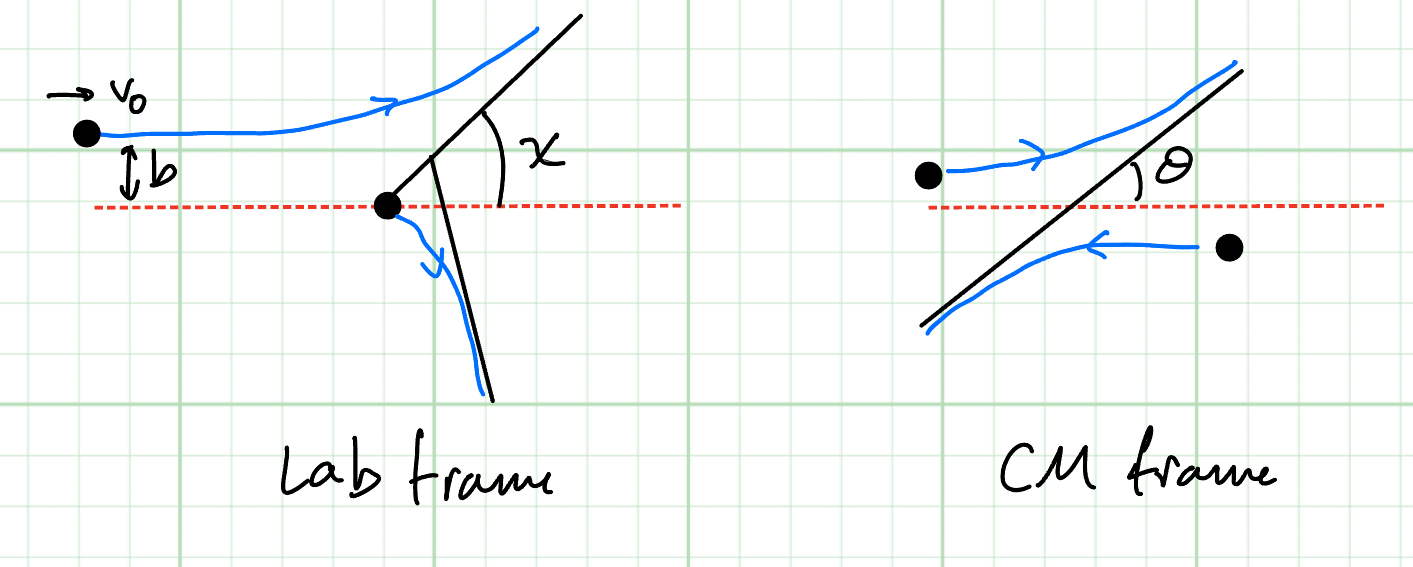
\includegraphics[width=\textwidth]{xsec-frames.jpeg}
    \caption{Definition of the physical setup and quantities relevant to the scattering of two particles interacting via a central potential in the lab frame (i.e. the target rest frame) and the center-of-mass frame.}
    \label{fig:scattering-setup}
\end{figure}

For the analytic result, although we are interested in the lab frame cross-section, it is easiest to first solve the two body problem in the center-of-mass (CM) frame and transform the results to the lab frame.
For brevity, we simply list the results of interest, skipping a detailed derivation, which can be found in essentially any classical mechanics textbook.
The outgoing angle 
%({\color{red} Check $v_0$ dependence. Should it be initial velocity in CM frame?})
\begin{align}
    \theta = 2 \arctan(\frac{\alpha Z_1 Z_2}{\mu b v_0^2})
,\end{align}
where $\mu = m_1 m_2 / (m_1 + m_2)$ is the reduced mass of the two-body system and $\alpha = e^2 / 4 \pi \epsilon_0$.
The CM frame cross section
\begin{align}
    \dv{\sigma}{\Omega_{\rm CM}} = \Bigg( \frac{\alpha Z_1 Z_2}{2 \mu v_0^2 \sin^2(\theta/2)} \Bigg)^2
.\end{align}
This result can be transformed into the lab frame cross section by observing that the scattering angles of the particle in the lab and CM frame, $\chi$ and $\theta$, respectively, are related through
\begin{align}
    \tan{\chi} = \frac{\sin{\theta}}{\cos{\theta} + \lambda}
,\end{align}
where $\lambda = m_1/m_2$.
The lab frame cross section
\begin{align}
    \dv{\sigma}{\Omega_{\rm lab}} = \Bigg| \dv{(\cos{\theta})}{(\cos{\chi})} \Bigg| \dv{\sigma}{\Omega_{\rm CM}} = \frac{(1 + 2 \lambda \cos{\theta} + \lambda^2)^{3/2}}{1 + \cos{\theta}} \dv{\sigma}{\Omega_{\rm CM}}
.\end{align}


\section{Numerical framework}
\label{sec:numerical-framework}

To compute the lab frame cross section, we adopt the following process.
We first simulate the motion of our particles, which requires solving the coupled set of second order differential equations, specified by Newton's 2$^{\rm nd}$ law:
\begin{align}
\begin{cases}
    \displaystyle m_1 \dv[2]{\vb*{r}_{1}}{t} = \vb*{F}_{1}(\vb*{r}_{1},\vb*{r}_{2}) \\
    \displaystyle m_2 \dv[2]{\vb*{r}_{2}}{t} = \vb*{F}_{2}(\vb*{r}_{1},\vb*{r}_{2})
,\end{cases}
\end{align}
where $\vb*{F}_{1} = - \grad_{1} V(\vb*{r}_{1},\vb*{r}_{2})$ is the Coulomb force on particle $1$ applied by particle 2 and similarly for $\vb*{F}_{2}$.
While we can implement a method which solves this second order equation for the position directly, it is useful to have velocities in hand for the computation of scattering angles.
Thus, we transform these second order equations into first order equations as follows:
\begin{align}
\begin{cases}
    \displaystyle \dv{\vb*{r}_{1}}{t} = \vb*{v}_{1} \\
    \displaystyle \dv{\vb*{v}_{1}}{t} = \frac{1}{m_1} \vb*{F}_{1}(\vb*{r}_{1},\vb*{r}_{2}) \\
    \displaystyle \dv{\vb*{r}_{2}}{t} = \vb*{v}_{2} \\
    \displaystyle \dv{\vb*{v}_{2}}{t} = \frac{1}{m_2} \vb*{F}_{2}(\vb*{r}_{1},\vb*{r}_{2})
.\end{cases}
\end{align}

These equations are solved using the RKF45 method with an adaptive step size, which generalizes quite simply from the one-dimensional case described in HW 5 by defining the state vector
\begin{align}
    \underline{q} = ( \vb*{r}_{1}, \vb*{v}_{1}, \vb*{r}_{2}, \vb*{v}_{2} )
.\end{align}
This state vector obeys the first order differential equation
\begin{align}
    \dv{\underline{q}}{t} = f(\underline{q},t)
,\end{align}
where
\begin{align}
    f(\underline{q},t) = ( \vb*{v}_{1}, \vb*{F}_{1}/m_1, \vb*{v}_{2}, \vb*{F}_{2}/m_2 )
.\end{align}
Note that in each iteration step we obtain a vector of errors, one for each quantity in the state vector, and we ensure that all of these is below the tolerance before accepting an iteration.

Once the particle motion is fully simulated, we must compute the scattering angle $\chi$ as
\begin{align}
    \chi = \arctan(\frac{v_{y,f}}{v_{x,f}})
,\end{align}
where $v_{x/y,f}$ are the $x$/$y$-components of the final velocity obtained by the differential equation solver.
Since we want to compute this angle accurately, we implement a condition which terminates the simulation as follows.
We first check that the relative or absolute difference between the angles $\chi_{n}$ and $\chi_{n+1}$ of subsequent steps are within some specified tolerances.
Additionally, since the incoming particle's motion is constructed to be nearly linear initially, we check that $|\vb*{r}_{1} - \vb*{r}_{2}| > |\vb*{r}_{1} - \vb*{r}_{2}|_{t = 0}$.
These two conditions must hold simultaneously before our simulation is terminated and a scattering angle is computed.

From this angle, we compute the derivative
\begin{align}
    \dv{b}{\chi} = \Big( \dv{\chi}{b} \Big)^{-1} = \ln(10) b \Bigg( \dv{\theta}{(\log_{10}(b))} \Bigg)^{-1}
\end{align}
using a finite difference method.
Note that we compute the derivative with respect to the transformed impact paramter $\log_{10}(b)$ since we initialize our array of impact parameters to be equally spaced in log-space.
For the first and last points in our $(\theta,\log_{10}(b))$ curve, we use the forward and backward central difference formulas
\begin{align}
    \theta'(\log_{10}(b_1)) &= \frac{\theta(\log_{10}(b_2)) - \theta(\log_{10}(b_1))}{\Delta(\log_{10}(b))} \\
    \theta'(\log_{10}(b_N)) &= \frac{\theta(\log_{10}(b_N)) - \theta(\log_{10}(b_{N-1}))}{\Delta(\log_{10}(b))}
,\end{align}
respectively.
For all other points, we use a central difference formula
\begin{align}
    \theta'(\log_{10}(b_n)) &= \frac{\theta(\log_{10}(b_{n+1})) - \theta(\log_{10}(b_{n-1}))}{2 \Delta(\log_{10}(b))}
.\end{align}
With this derivative in hand, we can compute the cross section as specified in Eq. \ref{eq:lab-cross-section}.


\section{Results}
\label{sec:results}

As a first pass to test the code, we analyze the case where our target particle is very massive.
In this case, $m_2 \rightarrow \infty$, $\mu \rightarrow m_1$, and $\chi \approx \theta$.
Thus, the lab/target rest frame and center-of-mass frame coincide.
In Fig. \ref{fig:test-solver}, we show the results of a simulation with impact parameter $b = 3$ and initial velocity $v_0 = 1$.
Note that in this work we set $\alpha = 1$ and all other quantities are referred to in some resulting arbitrary units.
We observe the classic trajectory of our scattered particle in the left-most panel.
Additionally, we see that energy is time-independent within machine precision as expected in the center panel.
Finally, in the right-most panel, we plot the angular momentum of the incoming particle relative to the origin.
We can see that this quantity is not conserved in our simulation, which does indeed violate our laws of physics since our potential is a central one, and therefore, there is no torque on the incoming particle at any time.

\begin{figure}[h!tb]
    \centering
    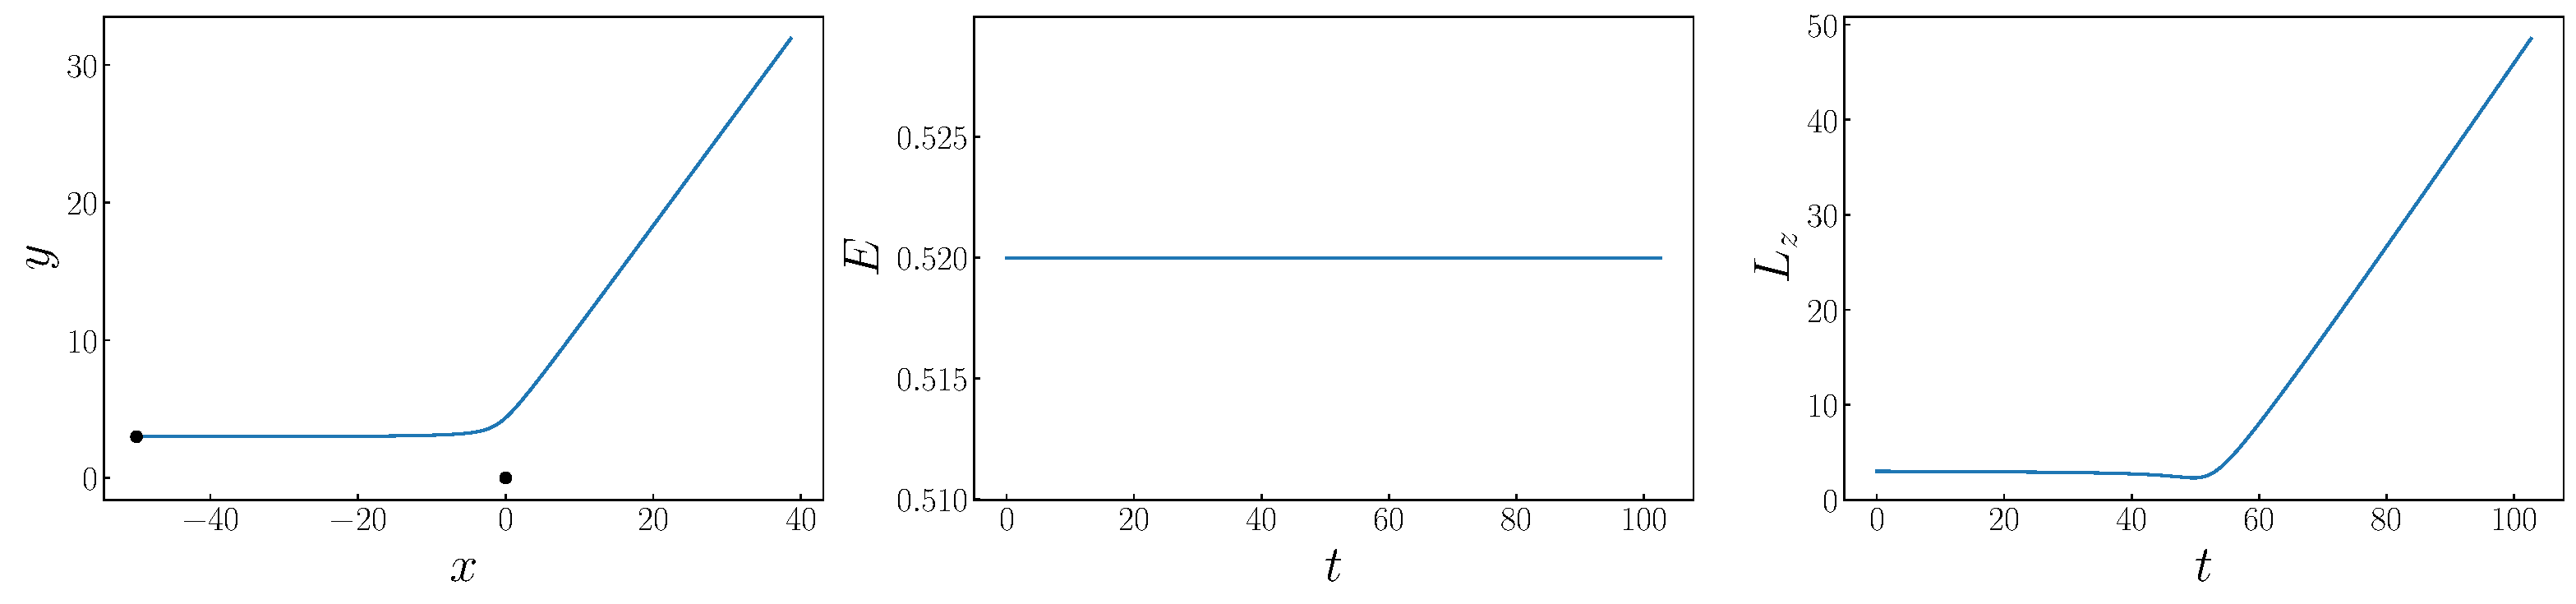
\includegraphics[width=\textwidth]{test_solver.pdf}
    \caption{[\textbf{Left}] Plot of the trajectory of an incoming particle of mass $m_1 = 1$ and a stationary target particle ($m_2 \rightarrow \infty$) with $Z_1 = Z_2 = 1$. [\textbf{Center}] Plot of the corresponding total mechanical energy of the system of particles as a function of time. [\textbf{Right}] Plot of the corresponding total angular momentum of the system of interacting particles as a function of time.}
    \label{fig:test-solver}
\end{figure}


In Fig. \ref{fig:part1-xsec}, we plot the scattering angle as a function of impact parameter for a proton scattering from a very heavy nucleus and the corresponding differential cross section.
We can see quite good agreement for small impact parameters and larger angles, which corresponds to results in the cross section which agree quite well at larger angles.
At smaller angles of deflection, although our simulation produces results which agree with the analytic solution regarding the angle but diverge from the analytic cross section a bit.
This may indicate some inaccuracies in our finite difference calculation of the derivative.


\begin{figure}[h!tb]
    \centering
    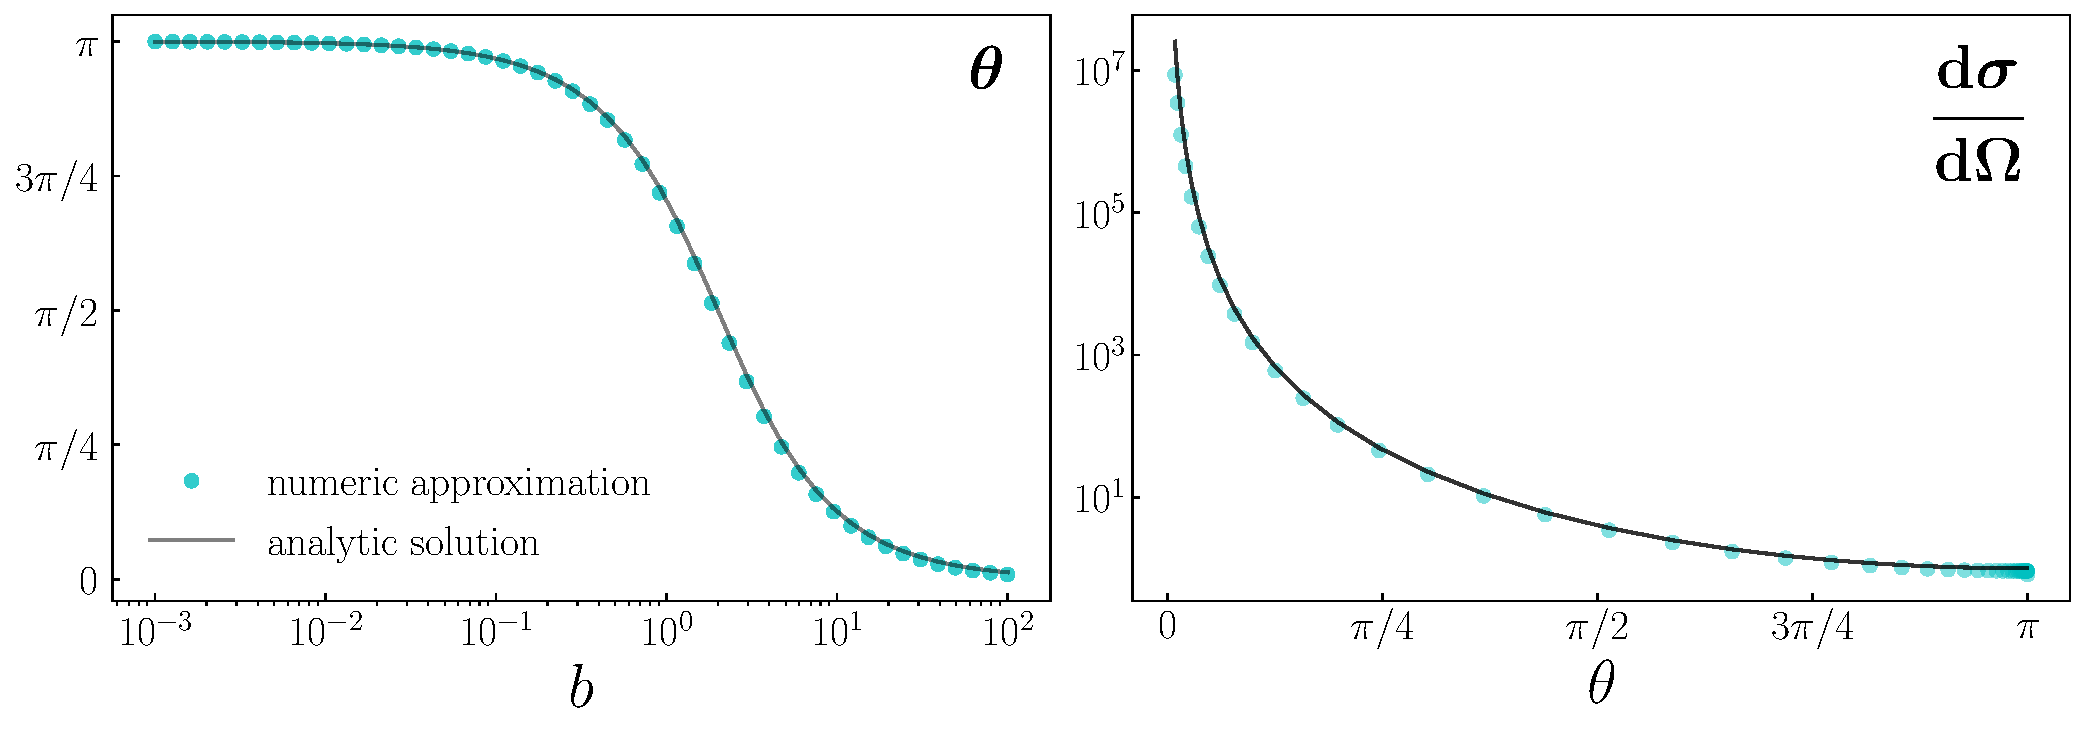
\includegraphics[width=\textwidth]{part1-xsec.pdf}
    \caption{[\textbf{Left}] Plot of the scattering angle for a proton ($m_1 = 1$, $Z_1 = 1$) scattering from a heavy nucleus ($m_2 \rightarrow \infty$) with $Z_2 = 2$ as a function of the impact paramter $b$. [\textbf{Right}] Plot of the differential cross section as a function of the scattering angle for the same scattering scenario described in the left plot.}
    \label{fig:part1-xsec}
\end{figure}

In Figs. \ref{fig:test-solver2} and \ref{fig:part2-xsec}, we simulate the scattering with particles of comparable masses, where the CM and lab frame scattering angles are no longer the same, and we therefore require the appropriate angle transformations and Jacobian factors on the cross section.
In Fig. \ref{fig:test-solver2}, we repeat the exercise of Fig. \ref{fig:test-solver}, plotting the trajectory simulated with $b = 2$ and $v_0 = 1$ for masses $m_1 = m_2 = Z_1 = Z_2 = 1$.
Again, we can see that the total mechanical energy of the system is essentially constant as a function of time, but the angular momentum of the system is not conserved, violating a fundamental law of physics.


\begin{figure}[h!tb]
    \centering
    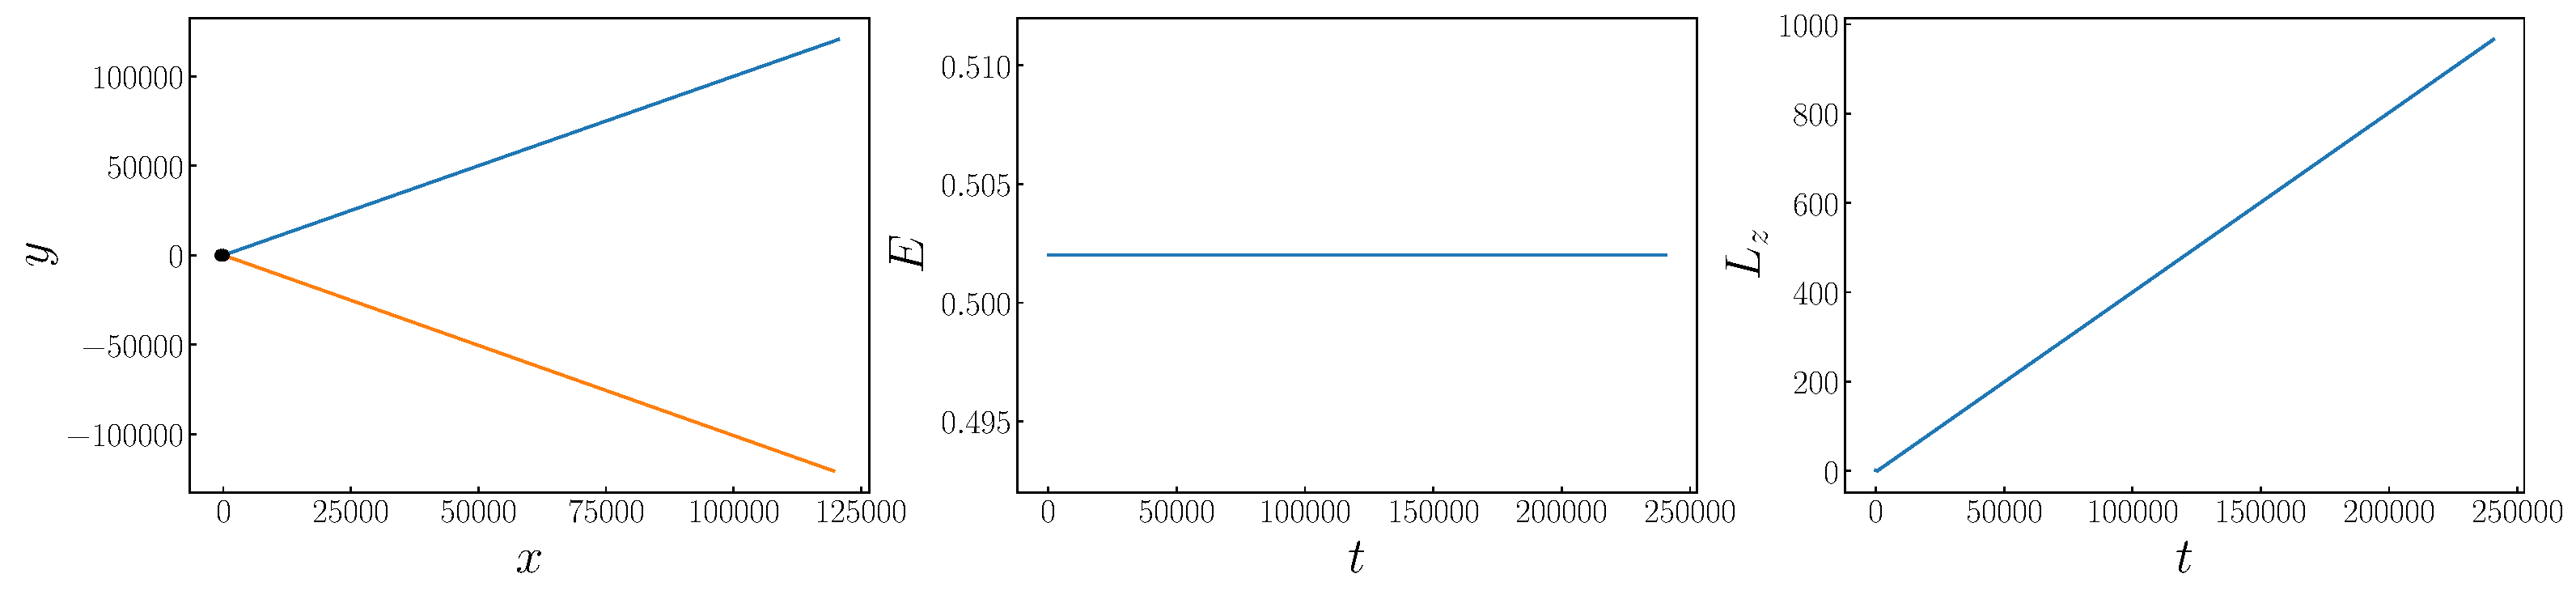
\includegraphics[width=\textwidth]{test_solver2.pdf}
    \caption{[\textbf{Left}] Plot of the trajectory of an incoming particle of mass $m_1 = 1$ and and initially at rest target particle with $m_2 = 1$ with $Z_1 = Z_2 = 1$. [\textbf{Center}] Plot of the corresponding total mechanical energy of the system of particles as a function of time. [\textbf{Right}] Plot of the corresponding total angular momentum of the system of interacting particles as a function of time.}
    \label{fig:test-solver2}
\end{figure}


In Fig. \ref{fig:part2-xsec}, we plot the lab frame scattering angle and cross section for proton's scattering from $\alpha$-particles as functions of the impact parameter and lab frame scattering angle, respectively.
In this case, we find reasonably good agreement between numerical approximations and analytic results across the space of impact parameters and scattering angles.

\begin{figure}[h!tb]
    \centering
    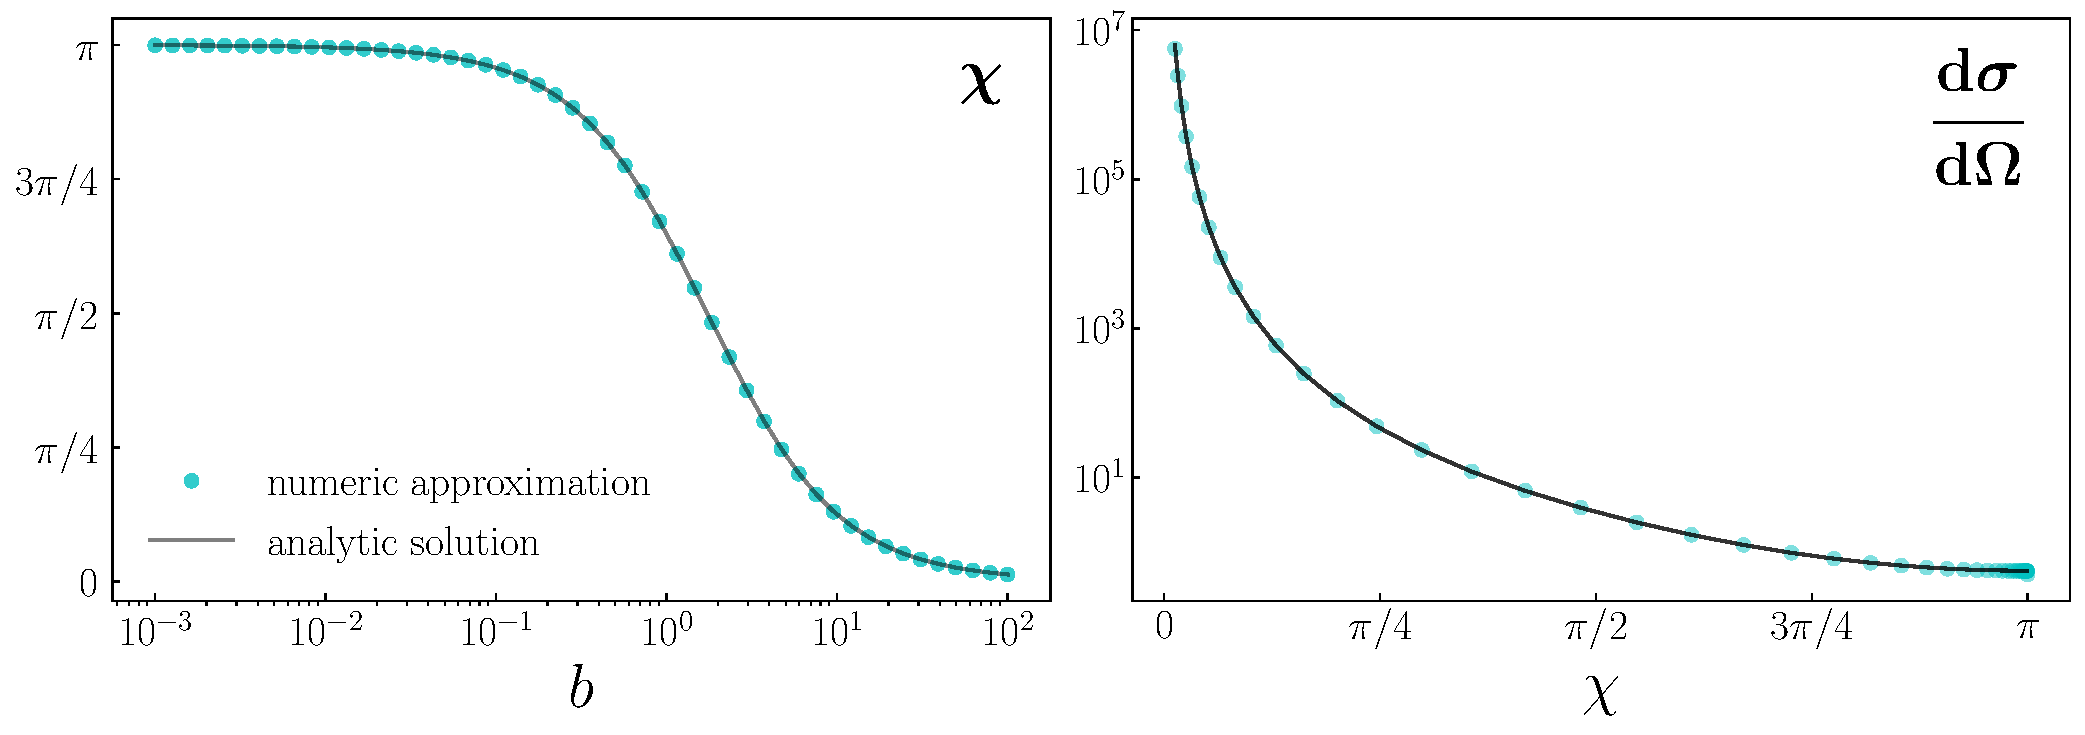
\includegraphics[width=\textwidth]{part2-xsec.pdf}
    \caption{[\textbf{Left}] Plot of the scattering angle for a proton ($m_1 = 1$, $Z_1 = 1$) scattering from an $\alpha$-particle ($m_2 = 2$, $Z_2 = 2$) as a function of the impact paramter $b$. [\textbf{Right}] Plot of the differential cross section in the lab frame as a function of the scattering angle for the same scattering scenario described in the left plot.}
    \label{fig:part2-xsec}
\end{figure}


\section{Conclusion}
\label{sec:conclusion}

We have endeavored in this project to implement some numerical techniques learned and explored in previous homework problems by calculating Rutherford scattering cross sections for cases with a heavy target, in which the lab and CM frames coincide, as well as those with incoming and target particles of comparable masses, where corrections must be made.
Across many physical scenarios, we find reasonable agreement, although in some cases, we can make improvements.
While the scattering angles are reconstructed well across most impact parameters but suffers a bit for very small impact parameters.
These behaviors are directly attributable to the numerical scheme.
When the impact parameter is larger, the forces are smaller, and therefore, it is easier to construct the trajectories for the particles, while on the other hand, it is more difficult to do so when the impact parameter is smaller.
When we go to construct the cross sections, while we find good results at intermediate scattering angles, the errors tend to be a bit larger at the end points, which seems more attributable to the finite difference scheme implemented to calculate the derivatives.

There are several ways that these results could be improved.
Firstly, we could make more careful choices with our parameters such as the step sizes or error tolerances.
Additionally, in order to address the lack of conservation of momentum, which is related to a fundamental symmetry, we could implement a scheme designed for particle dynamics.
In either case, it is crucial that our numerical methods yield robust, accurate results since scattering experiments are some of the most common ways we learn about the structure of particles and the interactions between them, and in most cases, we cannot obtain closed form analytic results for the lab frame differential cross sections.


    
\end{document}
